\documentclass[tikz,border=10pt]{standalone}
\usepackage{tikz}
\usepackage{amsmath,amssymb}
\usepackage{xcolor}
\usetikzlibrary{decorations.markings,arrows.meta,calc,positioning,shapes,backgrounds,patterns}

% Color scheme - professional physics journal style
\definecolor{anyonblue}{RGB}{41,128,185}
\definecolor{anyonred}{RGB}{192,57,43}
\definecolor{anyongreen}{RGB}{39,174,96}
\definecolor{anyonpurple}{RGB}{142,68,173}
\definecolor{anyonorange}{RGB}{230,126,34}
\definecolor{fusionbg}{RGB}{248,249,250}
\definecolor{vacuumgray}{RGB}{149,165,166}

\begin{document}

% ===========================================
% FIGURE: Anyon Braiding Worldlines
% ===========================================
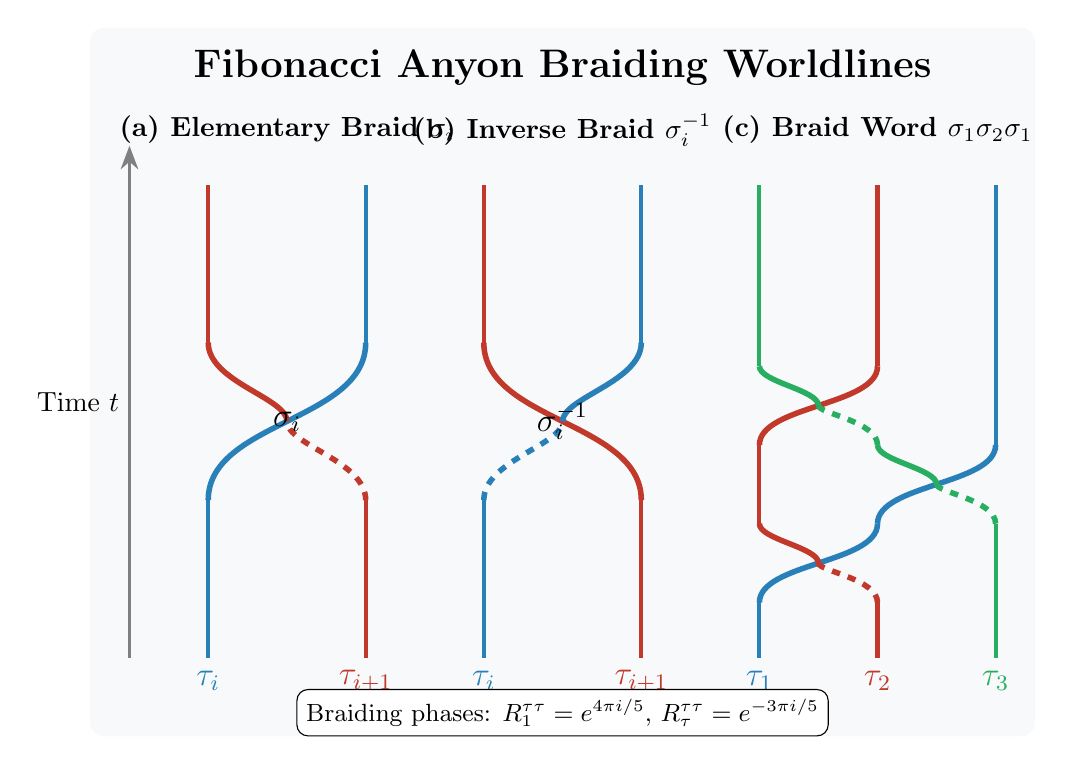
\begin{tikzpicture}[
    worldline/.style={line width=1.5pt},
    braid/.style={line width=2pt},
    time arrow/.style={-{Stealth[length=3mm]}, thick, gray},
    anyon label/.style={font=\large\bfseries}
]

% Background
\fill[fusionbg, rounded corners=5pt] (-1,-0.5) rectangle (11,8.5);

% Title
\node[font=\Large\bfseries] at (5,8) {Fibonacci Anyon Braiding Worldlines};

% Time arrow
\draw[time arrow] (-0.5,0.5) -- (-0.5,7) node[midway, left, black] {Time $t$};

% === Panel (a): Single braid σ_i ===
\node[font=\bfseries] at (1.5,7.2) {(a) Elementary Braid $\sigma_i$};

% Worldlines - particle i crosses over particle i+1
\draw[worldline, anyonblue] (0.5,0.5) -- (0.5,2.5);
\draw[worldline, anyonred] (2.5,0.5) -- (2.5,2.5);

% The braid crossing
\draw[braid, anyonblue] (0.5,2.5) .. controls (0.5,3.5) and (2.5,3.5) .. (2.5,4.5);
\draw[braid, anyonred, dashed] (2.5,2.5) .. controls (2.5,3) and (1.5,3.2) .. (1.5,3.5);
\draw[braid, anyonred] (1.5,3.5) .. controls (1.5,3.8) and (0.5,4) .. (0.5,4.5);

% Continue worldlines
\draw[worldline, anyonblue] (2.5,4.5) -- (2.5,6.5);
\draw[worldline, anyonred] (0.5,4.5) -- (0.5,6.5);

% Anyon labels
\node[anyon label, anyonblue] at (0.5,0.2) {$\tau_i$};
\node[anyon label, anyonred] at (2.5,0.2) {$\tau_{i+1}$};

% Braid label
\node[font=\large] at (1.5,3.5) {$\sigma_i$};

% === Panel (b): Inverse braid σ_i^{-1} ===
\node[font=\bfseries] at (5,7.2) {(b) Inverse Braid $\sigma_i^{-1}$};

% Worldlines
\draw[worldline, anyonblue] (4,0.5) -- (4,2.5);
\draw[worldline, anyonred] (6,0.5) -- (6,2.5);

% The inverse braid crossing (opposite handedness)
\draw[braid, anyonred] (6,2.5) .. controls (6,3.5) and (4,3.5) .. (4,4.5);
\draw[braid, anyonblue, dashed] (4,2.5) .. controls (4,3) and (5,3.2) .. (5,3.5);
\draw[braid, anyonblue] (5,3.5) .. controls (5,3.8) and (6,4) .. (6,4.5);

% Continue worldlines
\draw[worldline, anyonred] (4,4.5) -- (4,6.5);
\draw[worldline, anyonblue] (6,4.5) -- (6,6.5);

% Anyon labels
\node[anyon label, anyonblue] at (4,0.2) {$\tau_i$};
\node[anyon label, anyonred] at (6,0.2) {$\tau_{i+1}$};

% Braid label
\node[font=\large] at (5,3.5) {$\sigma_i^{-1}$};

% === Panel (c): Braid word σ_1 σ_2 σ_1 ===
\node[font=\bfseries] at (9,7.2) {(c) Braid Word $\sigma_1\sigma_2\sigma_1$};

% Three anyons
\draw[worldline, anyonblue] (7.5,0.5) -- (7.5,1.2);
\draw[worldline, anyonred] (9,0.5) -- (9,1.2);
\draw[worldline, anyongreen] (10.5,0.5) -- (10.5,1.2);

% First braid σ_1
\draw[braid, anyonblue] (7.5,1.2) .. controls (7.5,1.7) and (9,1.7) .. (9,2.2);
\draw[braid, anyonred, dashed] (9,1.2) .. controls (9,1.5) and (8.25,1.6) .. (8.25,1.7);
\draw[braid, anyonred] (8.25,1.7) .. controls (8.25,1.9) and (7.5,2) .. (7.5,2.2);
\draw[worldline, anyongreen] (10.5,1.2) -- (10.5,2.2);

% Second braid σ_2
\draw[worldline, anyonred] (7.5,2.2) -- (7.5,3.2);
\draw[braid, anyonblue] (9,2.2) .. controls (9,2.7) and (10.5,2.7) .. (10.5,3.2);
\draw[braid, anyongreen, dashed] (10.5,2.2) .. controls (10.5,2.5) and (9.75,2.6) .. (9.75,2.7);
\draw[braid, anyongreen] (9.75,2.7) .. controls (9.75,2.9) and (9,3) .. (9,3.2);

% Third braid σ_1
\draw[braid, anyonred] (7.5,3.2) .. controls (7.5,3.7) and (9,3.7) .. (9,4.2);
\draw[braid, anyongreen, dashed] (9,3.2) .. controls (9,3.5) and (8.25,3.6) .. (8.25,3.7);
\draw[braid, anyongreen] (8.25,3.7) .. controls (8.25,3.9) and (7.5,4) .. (7.5,4.2);
\draw[worldline, anyonblue] (10.5,3.2) -- (10.5,4.2);

% Final worldlines
\draw[worldline, anyongreen] (7.5,4.2) -- (7.5,6.5);
\draw[worldline, anyonred] (9,4.2) -- (9,6.5);
\draw[worldline, anyonblue] (10.5,4.2) -- (10.5,6.5);

% Anyon labels
\node[anyon label, anyonblue] at (7.5,0.2) {$\tau_1$};
\node[anyon label, anyonred] at (9,0.2) {$\tau_2$};
\node[anyon label, anyongreen] at (10.5,0.2) {$\tau_3$};

% R-matrix annotation
\node[draw, rounded corners, fill=white, font=\small] at (5,-0.2) {
    Braiding phases: $R_1^{\tau\tau} = e^{4\pi i/5}$, $R_\tau^{\tau\tau} = e^{-3\pi i/5}$
};

\end{tikzpicture}

\newpage

% ===========================================
% FIGURE: Fusion Tree Diagrams
% ===========================================
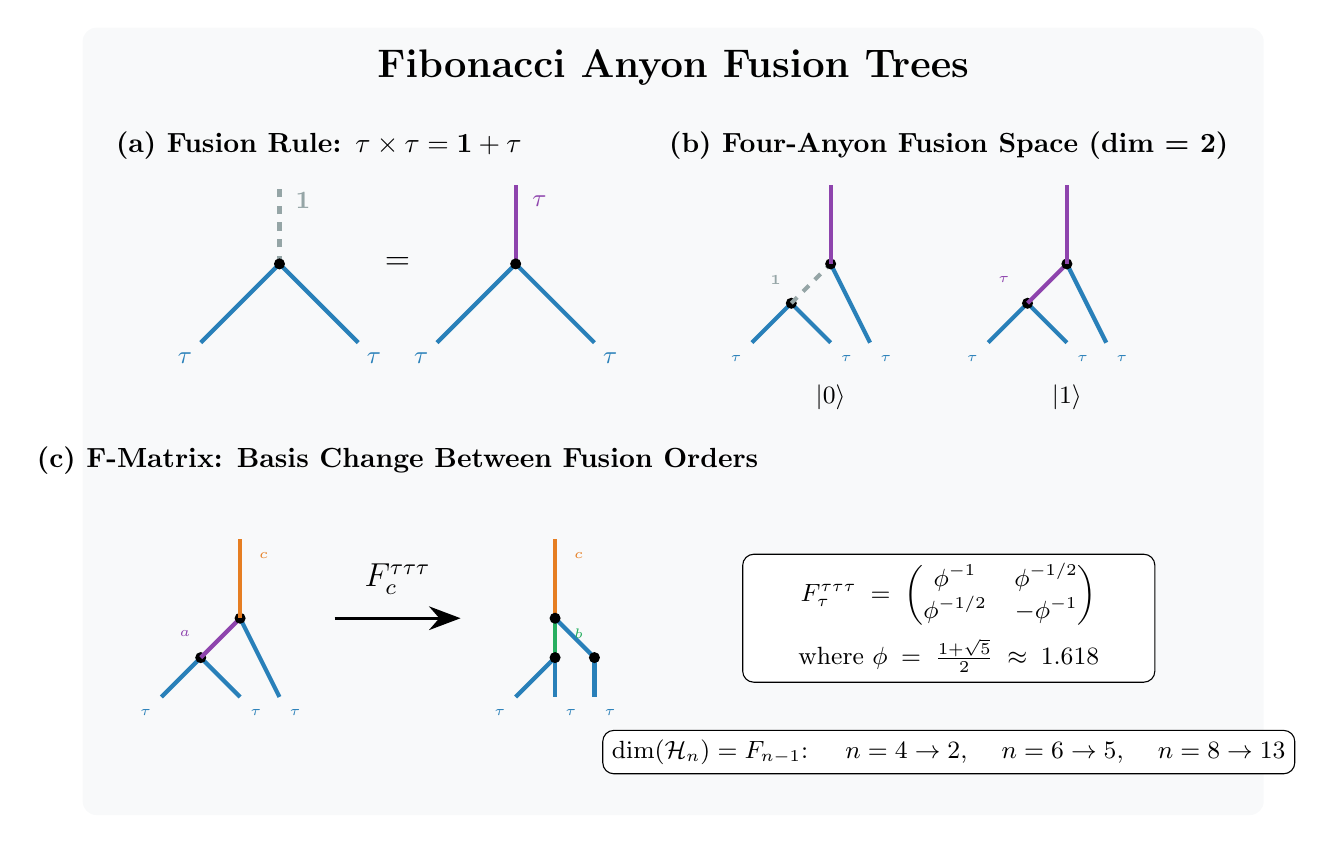
\begin{tikzpicture}[
    fusion line/.style={line width=1.5pt},
    vertex/.style={circle, fill=black, minimum size=4pt, inner sep=0pt},
    charge label/.style={font=\small\bfseries, midway},
    tree bg/.style={fill=fusionbg, rounded corners=5pt}
]

% Background
\fill[fusionbg, rounded corners=5pt] (-1,-1) rectangle (14,9);

% Title
\node[font=\Large\bfseries] at (6.5,8.5) {Fibonacci Anyon Fusion Trees};

% === Panel (a): Basic fusion τ × τ = 1 + τ ===
\node[font=\bfseries] at (2,7.5) {(a) Fusion Rule: $\tau \times \tau = \mathbf{1} + \tau$};

% Fusion to vacuum
\draw[fusion line, anyonblue] (0.5,5) -- (1.5,6);
\draw[fusion line, anyonblue] (2.5,5) -- (1.5,6);
\draw[fusion line, vacuumgray, dashed] (1.5,6) -- (1.5,7);
\node[vertex] at (1.5,6) {};
\node[anyonblue, font=\small\bfseries] at (0.3,4.8) {$\tau$};
\node[anyonblue, font=\small\bfseries] at (2.7,4.8) {$\tau$};
\node[vacuumgray, font=\small\bfseries] at (1.8,6.8) {$\mathbf{1}$};

% Fusion to tau
\draw[fusion line, anyonblue] (3.5,5) -- (4.5,6);
\draw[fusion line, anyonblue] (5.5,5) -- (4.5,6);
\draw[fusion line, anyonpurple] (4.5,6) -- (4.5,7);
\node[vertex] at (4.5,6) {};
\node[anyonblue, font=\small\bfseries] at (3.3,4.8) {$\tau$};
\node[anyonblue, font=\small\bfseries] at (5.7,4.8) {$\tau$};
\node[anyonpurple, font=\small\bfseries] at (4.8,6.8) {$\tau$};

% Equation
\node[font=\large] at (3,6) {$=$};

% === Panel (b): Four-anyon fusion tree ===
\node[font=\bfseries] at (10,7.5) {(b) Four-Anyon Fusion Space (dim = 2)};

% Tree 1: ((τ×τ)_1 × τ) = τ
\draw[fusion line, anyonblue] (7.5,5) -- (8,5.5);
\draw[fusion line, anyonblue] (8.5,5) -- (8,5.5);
\node[vertex] at (8,5.5) {};
\draw[fusion line, vacuumgray, dashed] (8,5.5) -- (8.5,6);
\draw[fusion line, anyonblue] (9,5) -- (8.5,6);
\node[vertex] at (8.5,6) {};
\draw[fusion line, anyonpurple] (8.5,6) -- (8.5,7);

\node[anyonblue, font=\tiny] at (7.3,4.8) {$\tau$};
\node[anyonblue, font=\tiny] at (8.7,4.8) {$\tau$};
\node[anyonblue, font=\tiny] at (9.2,4.8) {$\tau$};
\node[vacuumgray, font=\tiny] at (7.8,5.8) {$\mathbf{1}$};
\node[font=\small] at (8.5,4.3) {$|0\rangle$};

% Tree 2: ((τ×τ)_τ × τ) = 1 or τ
\draw[fusion line, anyonblue] (10.5,5) -- (11,5.5);
\draw[fusion line, anyonblue] (11.5,5) -- (11,5.5);
\node[vertex] at (11,5.5) {};
\draw[fusion line, anyonpurple] (11,5.5) -- (11.5,6);
\draw[fusion line, anyonblue] (12,5) -- (11.5,6);
\node[vertex] at (11.5,6) {};
\draw[fusion line, anyonpurple] (11.5,6) -- (11.5,7);

\node[anyonblue, font=\tiny] at (10.3,4.8) {$\tau$};
\node[anyonblue, font=\tiny] at (11.7,4.8) {$\tau$};
\node[anyonblue, font=\tiny] at (12.2,4.8) {$\tau$};
\node[anyonpurple, font=\tiny] at (10.7,5.8) {$\tau$};
\node[font=\small] at (11.5,4.3) {$|1\rangle$};

% === Panel (c): F-matrix basis change ===
\node[font=\bfseries] at (3,3.5) {(c) F-Matrix: Basis Change Between Fusion Orders};

% Left tree
\draw[fusion line, anyonblue] (0,0.5) -- (0.5,1);
\draw[fusion line, anyonblue] (1,0.5) -- (0.5,1);
\node[vertex] at (0.5,1) {};
\draw[fusion line, anyonpurple] (0.5,1) -- (1,1.5);
\draw[fusion line, anyonblue] (1.5,0.5) -- (1,1.5);
\node[vertex] at (1,1.5) {};
\draw[fusion line, anyonorange] (1,1.5) -- (1,2.5);

\node[anyonblue, font=\tiny] at (-0.2,0.3) {$\tau$};
\node[anyonblue, font=\tiny] at (1.2,0.3) {$\tau$};
\node[anyonblue, font=\tiny] at (1.7,0.3) {$\tau$};
\node[anyonpurple, font=\tiny] at (0.3,1.3) {$a$};
\node[anyonorange, font=\tiny] at (1.3,2.3) {$c$};

% Arrow with F-matrix
\draw[-{Stealth[length=4mm]}, very thick] (2.2,1.5) -- (3.8,1.5);
\node[font=\large] at (3,2) {$F^{\tau\tau\tau}_c$};

% Right tree
\draw[fusion line, anyonblue] (4.5,0.5) -- (5,1);
\draw[fusion line, anyonblue] (5.5,0.5) -- (5.5,1);
\draw[fusion line, anyonblue] (5.5,1) -- (5,1.5);
\node[vertex] at (5.5,1) {};
\draw[fusion line, anyonblue] (5,0.5) -- (5,1);
\draw[fusion line, anyongreen] (5,1) -- (5,1.5);
\node[vertex] at (5,1) {};
\draw[fusion line, anyonorange] (5,1.5) -- (5,2.5);
\node[vertex] at (5,1.5) {};

\node[anyonblue, font=\tiny] at (4.3,0.3) {$\tau$};
\node[anyonblue, font=\tiny] at (5.2,0.3) {$\tau$};
\node[anyonblue, font=\tiny] at (5.7,0.3) {$\tau$};
\node[anyongreen, font=\tiny] at (5.3,1.3) {$b$};
\node[anyonorange, font=\tiny] at (5.3,2.3) {$c$};

% F-matrix explicit
\node[draw, rounded corners, fill=white, font=\small, text width=5cm, align=center] at (10,1.5) {
    $F^{\tau\tau\tau}_\tau = \begin{pmatrix} \phi^{-1} & \phi^{-1/2} \\ \phi^{-1/2} & -\phi^{-1} \end{pmatrix}$\\[3pt]
    where $\phi = \frac{1+\sqrt{5}}{2} \approx 1.618$
};

% Dimension formula
\node[draw, rounded corners, fill=white, font=\small] at (10,-0.2) {
    $\dim(\mathcal{H}_n) = F_{n-1}$: \quad $n=4 \to 2$, \quad $n=6 \to 5$, \quad $n=8 \to 13$
};

\end{tikzpicture}

\newpage

% ===========================================
% FIGURE: TQRC Architecture (Professional)
% ===========================================
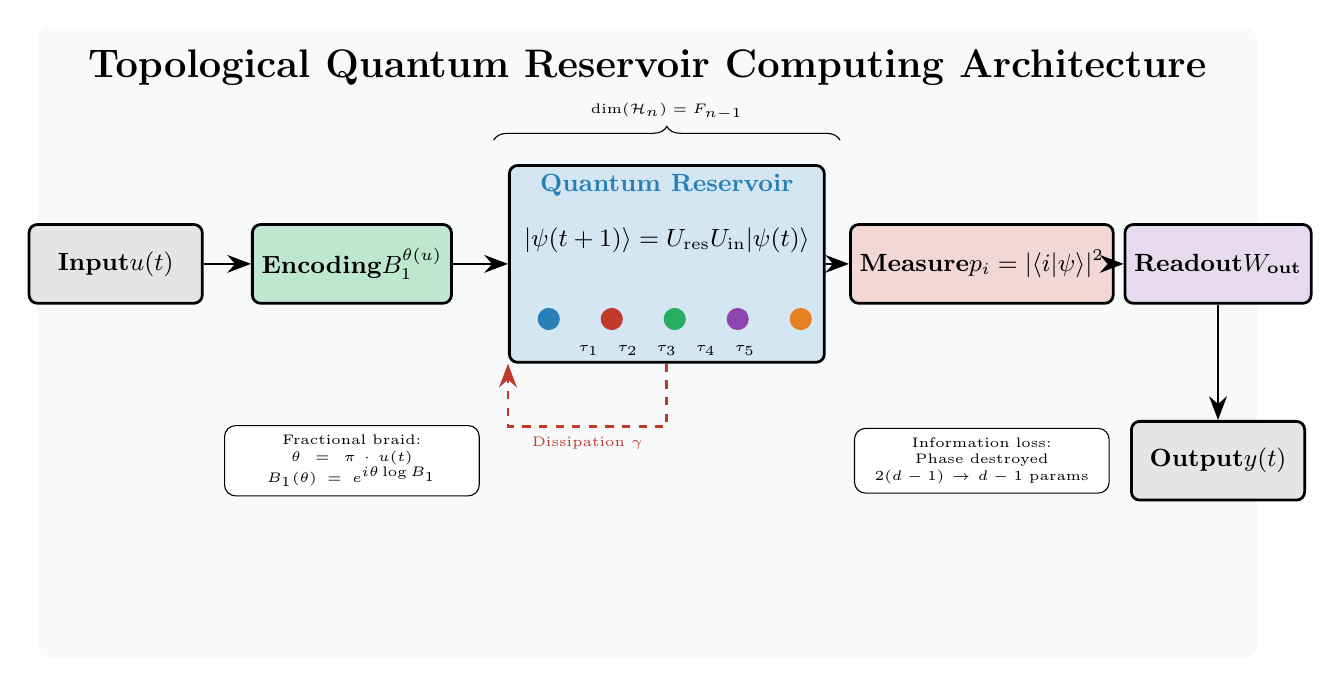
\begin{tikzpicture}[
    block/.style={draw, rounded corners=3pt, minimum width=2.2cm, minimum height=1cm, font=\small\bfseries, line width=1pt},
    arrow/.style={-{Stealth[length=3mm]}, line width=1pt},
    brace/.style={decorate, decoration={brace, amplitude=5pt, raise=2pt}}
]

% Background
\fill[fusionbg, rounded corners=5pt] (-0.5,-2) rectangle (15,6);

% Title
\node[font=\Large\bfseries] at (7.25,5.5) {Topological Quantum Reservoir Computing Architecture};

% Input
\node[block, fill=gray!20] (input) at (0.5,3) {Input\\$u(t)$};

% Encoding
\node[block, fill=anyongreen!30] (encode) at (3.5,3) {Encoding\\$B_1^{\theta(u)}$};

% Reservoir (larger, with anyons inside)
\node[block, fill=anyonblue!20, minimum width=4cm, minimum height=2.5cm] (reservoir) at (7.5,3) {};
\node[font=\small\bfseries, anyonblue] at (7.5,4) {Quantum Reservoir};
\node[font=\small] at (7.5,3.3) {$|\psi(t+1)\rangle = U_{\text{res}} U_{\text{in}} |\psi(t)\rangle$};

% Draw anyons inside reservoir
\foreach \x/\c in {6/anyonblue, 6.8/anyonred, 7.6/anyongreen, 8.4/anyonpurple, 9.2/anyonorange} {
    \fill[\c] (\x,2.3) circle (4pt);
}
\node[font=\tiny] at (7.5,1.9) {$\tau_1 \quad \tau_2 \quad \tau_3 \quad \tau_4 \quad \tau_5$};

% Measurement
\node[block, fill=anyonred!20] (measure) at (11.5,3) {Measure\\$p_i = |\langle i|\psi\rangle|^2$};

% Readout
\node[block, fill=anyonpurple!20] (readout) at (14.5,3) {Readout\\$W_{\text{out}}$};

% Output
\node[block, fill=gray!20] (output) at (14.5,0.5) {Output\\$y(t)$};

% Arrows
\draw[arrow] (input) -- (encode);
\draw[arrow] (encode) -- (reservoir.west);
\draw[arrow] (reservoir.east) -- (measure);
\draw[arrow] (measure) -- (readout);
\draw[arrow] (readout) -- (output);

% Feedback loop (optional dissipation)
\draw[arrow, dashed, anyonred] (reservoir.south) -- ++(0,-0.8) -| node[pos=0.25, below, font=\tiny] {Dissipation $\gamma$} (reservoir.south west);

% Annotations
\node[draw, rounded corners, fill=white, font=\tiny, text width=3cm, align=center] at (3.5,0.5) {
    Fractional braid:\\
    $\theta = \pi \cdot u(t)$\\
    $B_1(\theta) = e^{i\theta \log B_1}$
};

\node[draw, rounded corners, fill=white, font=\tiny, text width=3cm, align=center] at (11.5,0.5) {
    Information loss:\\
    Phase destroyed\\
    $2(d-1) \to d-1$ params
};

% Hilbert space dimension
\draw[brace] (5.3,4.5) -- (9.7,4.5);
\node[font=\tiny, above] at (7.5,4.7) {$\dim(\mathcal{H}_n) = F_{n-1}$};

\end{tikzpicture}

\newpage

% ===========================================
% FIGURE: Unitarity vs ESP Tension
% ===========================================
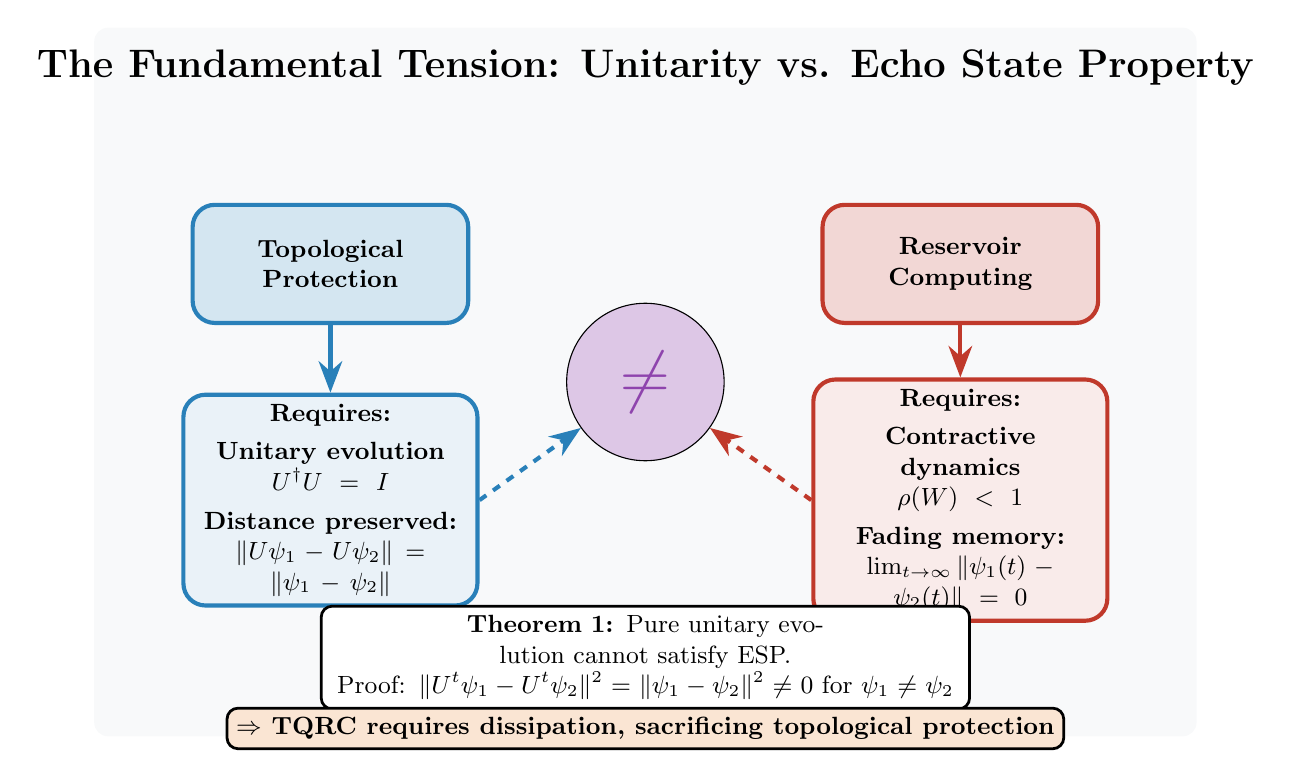
\begin{tikzpicture}[
    concept/.style={draw, rounded corners=8pt, minimum width=3.5cm, minimum height=1.5cm, font=\small\bfseries, line width=1.5pt, align=center},
    arrow/.style={-{Stealth[length=4mm]}, line width=1.5pt}
]

% Background
\fill[fusionbg, rounded corners=5pt] (-1,-1) rectangle (13,8);

% Title
\node[font=\Large\bfseries] at (6,7.5) {The Fundamental Tension: Unitarity vs. Echo State Property};

% Topological Protection (left)
\node[concept, fill=anyonblue!20, draw=anyonblue] (topo) at (2,5) {Topological\\Protection};

% Reservoir Computing (right)
\node[concept, fill=anyonred!20, draw=anyonred] (rc) at (10,5) {Reservoir\\Computing};

% Requirements
\node[concept, fill=anyonblue!10, draw=anyonblue, minimum height=2.5cm, text width=3.5cm] (unitary) at (2,2) {
    \textbf{Requires:}\\[3pt]
    Unitary evolution\\
    $U^\dagger U = I$\\[3pt]
    Distance preserved:\\
    $\|U\psi_1 - U\psi_2\| = \|\psi_1 - \psi_2\|$
};

\node[concept, fill=anyonred!10, draw=anyonred, minimum height=2.5cm, text width=3.5cm] (contract) at (10,2) {
    \textbf{Requires:}\\[3pt]
    Contractive dynamics\\
    $\rho(W) < 1$\\[3pt]
    Fading memory:\\
    $\lim_{t\to\infty}\|\psi_1(t) - \psi_2(t)\| = 0$
};

% Arrows from concepts to requirements
\draw[arrow, anyonblue] (topo) -- (unitary);
\draw[arrow, anyonred] (rc) -- (contract);

% Central conflict
\node[draw, circle, fill=anyonpurple!30, minimum size=2cm, font=\Huge\bfseries, text=anyonpurple] (conflict) at (6,3.5) {$\neq$};

% Conflict arrows
\draw[arrow, anyonblue, dashed] (unitary.east) -- (conflict);
\draw[arrow, anyonred, dashed] (contract.west) -- (conflict);

% Theorem box
\node[draw, rounded corners, fill=white, line width=1pt, font=\small, text width=8cm, align=center] at (6,0) {
    \textbf{Theorem 1:} Pure unitary evolution cannot satisfy ESP.\\
    Proof: $\|U^t\psi_1 - U^t\psi_2\|^2 = \|\psi_1 - \psi_2\|^2 \neq 0$ for $\psi_1 \neq \psi_2$
};

% Consequence
\node[draw, rounded corners, fill=anyonorange!20, line width=1pt, font=\small\bfseries] at (6,-0.9) {
    $\Rightarrow$ TQRC requires dissipation, sacrificing topological protection
};

\end{tikzpicture}

\end{document}
